\chapter{Introdução}

Este é o capítulo introdutório da monografia e está dividido em cinco seções. A primeira trata de descrever a motivação encontrada para a execução do corrente trabalho, a segunda contextualiza o ambiente e condições de aplicação e a terceira demonstra, em linhas gerais, a situação problema encontrada. Após isso, na quinta seção, as possíveis soluções existentes para o problema exposto são discutidas e, por fim, a estrutura da monografia é descrita.

\section{Motivação}

Todos os dias novos produtos surgem no mercado tecnológico com o objetivo de solucionar algum problema do cotidiano de empresas e instituições. O Sistema Gema, como sistema de informação, é proposto com o intuito lapidar processos diretamente relacionados com a criação de materiais didáticos, interesse cuja preocupação deve ser notória, pois, à medida que o produto da instituição é o ensino, a qualificação dos seus alunos deve ser seu carro chefe.

No Instituto Metrópole Digital, assim como nos demais institutos de ensino, os benefícios que os recursos tecnológicos presentes fornecem precisam ser melhor aproveitados. Para isso, a percepção do poder da tecnologia da informação e a adesão ao novo devem ser praticados. 

Este trabalho nada mais é do que a junção da prática desses comportamentos com a disposição e vontade do graduando de aplicar o conhecimento adquirido na instituição ao longo dos anos de estudo. O sistema aqui proposto é um modelo totalmente baseado nas necessidades do setor e que proporcionará o domínio dos processos produtivos e o aumento de performance do trabalho executado.

\section{Contextualização}

Como Unidade Suplementar da Universidade Federal do Rio Grande do Norte (UFRN), o Instituto Metrópole Digital (IMD) atua na formação de jovens e adultos de nível técnico, superior e pós-graduação. Suas ações integram a inclusão social e digital de estudantes do ensino básico à pós-graduação, a realização de pesquisa e inovação tecnológica e o incentivo à cultura do empreendedorismo.

Hoje o IMD encontra-se particionado em diversos setores, cada qual com seu objetivo e metodologia. Entre estes setores, está o setor de materiais, responsável pela produção de todo o material disponibilizado pelo instituto e principal interessado no desenvolvimento deste trabalho. 

Dentro do setor de materiais é possível extrair todos os fluxos que contemplam a criação de um material e, na figura a seguir, é possível entender como um dos principais fluxos funciona. \\

\vspace{5mm}
\begin{minipage}[c]{\textwidth}
    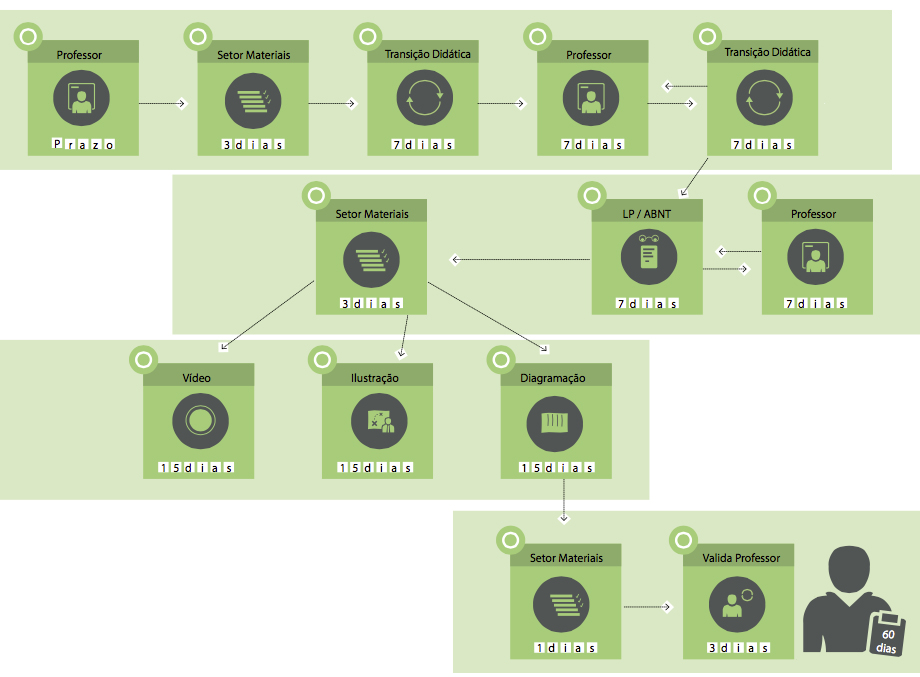
\includegraphics[width=14cm]{Imagens/FluxoMateriaisNovos.jpg}
    \captionof{figure}{Fluxo de Criação de Materiais Didáticos}
    \label{fig:fluxo_materiais_novos}
\end{minipage}
\vspace{5mm}

A \hyperref[fig:fluxo_materiais_novos]{Figura \ref{fig:fluxo_materiais_novos}} descreve o fluxo para a criação do material didático de uma aula. Ele é iniciado com o envio do arquivo pelo autor para o setor de materiais, onde será feita uma primeira análise do conteúdo do material, o qual é então repassado para a equipe pedagógica responsável pela transição didática, processo de adaptar os conteúdos à perspectiva pedagógica da instituição. O material então fica alternando de responsabilidade entre o professor e a equipe pedagógica até que essa última determine a conformidade do conteúdo. Neste momento, a equipe de língua portuguesa e normas ABNT recebe o arquivo e se encarrega por executar revisões e melhorias juntamente com o professor, o resultado é encaminhado ao setor de materiais que, de acordo com as necessidades, solicita criação de material de vídeo, ilustração e, por último, diagramação, processo de organizar o material para publicação. Quando a equipe de diagramação termina seu trabalho, o arquivo volta à coordenação do setor de materiais para que seja feita uma nova verificação nos resultados obtidos e seja solicitada aprovação do professor que iniciou o processo.

No fluxo descrito, algumas equipes foram citadas, cada uma dessas está representada na \hyperref[fig:fluxo_materiais_novos]{Figura \ref{fig:fluxo_materiais_novos}} por um bloco e destaca um envolvido no processo, alguns deles são subsetores do setor de materiais e outros externos a esse. Na tabela abaixo é possível entender suas funções.

\begin{center}
\captionof{table}{Definição de envolvidos e papéis}
\begin{tabular}{|p{3cm}|p{11cm}|}
\hline            
\rowcolor[HTML]{EFEFEF}      
\textbf{Nome} & \textbf{Papel} \\ \hline
Autor (professor) & Elabora o material de aula/prova na sua versão inicial e participa do fluxo realizando melhorias e correções.                                                                                               \\ \hline
Gerência           & O setor de materiais é principalmente responsável por auditar o processo de criação do material. Ele garante a execução dos passos do fluxo, o cumprimento dos prazos e a conformidade com as necessidades. \\ \hline
Transição Didática & Na transição didática há a formatação textual de acordo com as necessidades pedagógicas da instituição.                                                                                                     \\ \hline
LP / ABNT          & Garante que as normas ortográficas e técnicas sejam respeitadas no conteúdo do material.                                                                                                                    \\ \hline
Vídeo              & Realiza criação, gravação e edição dos vídeos necessários para preencher o material didático.                                                                                                               \\ \hline
Ilustração         & Responsável por toda a parte gráfica/artística dos materiais.                                                                                                                                               \\ \hline
Diagramação        & Define a organização final do material para a publicação.                                                                                                                                                   \\ \hline
\end{tabular}
\end{center}

\section{Situação Problema}

Os passos quem compõem o fluxo existem com intuito de gerar resultados. Esses resultados representam um produto, um material que possui valor para o instituto. 

Tomando como exemplo o fluxo de materiais didáticos novos (ver \hyperref[fig:fluxo_materiais_novos]{Figura \ref{fig:fluxo_materiais_novos}}), na prática, os passos executados acontecem da seguinte maneira:

\begin{enumerate}
  \item O autor (professor) envia os arquivos do material de aula à gerência do setor de materiais através de e-mail;
  \item Ao receber os arquivos, a equipe de gerência cria uma planilha com os dados do material, valida os documentos e passa para a equipe pedagógica;
  \item A equipe de pedagógica então executa a revisão textual e retorna para o autor caso seja necessário realizar ajustes. Esse ciclo se repete até que a equipe determine que o material está totalmente de acordo com as necessidades percebidas. Ao final, o material é enviado para a revisão de língua portuguesa e de normas ABNT;
  \item Os responsáveis pelas revisões LP/ABNT atuam sobre o material em conjunto com o autor até que os textos estejam em conformidade com as normas ortográficas e técnicas.
  \item O resultado do passo anterior é então encaminhado à gerência do setor que atualiza o estado do material na planilha e coordena os próximos passos. Neste momento, eles precisam determinar os elementos de audiovisual que são necessários para completar o produto. Essas necessidades resultam em solicitações para a equipe de vídeo, ilustração e, por último, diagramação. 
  \item Ao passo que a equipe de diagramação finaliza seu trabalho, há uma última verificação feita pela gerência e, então, todo o resultado retorna ao autor para a validação final.
\end{enumerate}

Durante o fluxo, a gerência utiliza de planilhas para administrar as versões do material e correio eletrônico para solicitações e conclusão das etapas. Em cada envio, a versão mais recente do material segue como anexo e, no corpo da mensagem, o direcionamento do que fazer e o prazo estipulado. Ao final do processo e dos e-mails trocados, o produto final se encontra pronto pra ser entregue aos alunos.

A forma como o processo descrito é executado representa a solução imediata encontrada pelos envolvidos para produção do material. Todavia, dado o estudo feito neste trabalho, é possível perceber que alguns pontos de falha se ressaltam nessa metodologia. 

Até o presente momento, foram citadas as utilizações de duas ferramentas importantes: o e-mail e a planilha. Como esses mecanismos não estão conectados diretamente, as suas utilizações implicam na necessidade de um forte mapeamento entre as solicitações e o acompanhamento da produção do material. Além disso, com a expansão das atividades e a elaboração de fluxos mais complexos, o número de envolvidos aumenta. Determinada equipe pode receber uma solicitação onde somente parte dos integrantes irá atuar sobre o material, o que gera outro nível de obrigação de controle, o interno da equipe. Por muitas vezes, os envolvidos precisam estar em contato direto, trocando informações e pedidos de maneira informal, o que descaracteriza o acompanhamento do método por parte da gerência. 

A perda de informação e registro causa não só a deficiência na execução quanto dificultam a criação de relatórios consistentes, pois há a necessidade de cruzamento manual de dados de diversas fontes. A equipe de gerência, responsável pela formação do material, tem o conhecimento prejudicado sobre o andamento do processo nas etapas das quais outras equipes são responsáveis. A ferramenta utilizada para as solicitações também pode facilitar a perda de prazos e de qualidade, visto que e-mails não propriamente enviados ou a não percepção do conteúdo que chega na caixa postal da equipe responsável pode acarretar em diminuição do tempo hábil para concretização do trabalho.

A contínua tarefa de verificação do recebimento do material e a necessidade de auditar o processo através de planilhas a parte dificultam a saída do material como o processo teoriza. 

Determinados os pontos de falha, caracterizamos a situação problema encontrada como base para a especificação e desenvolvimento do corrente trabalho.

\section{Estado da Arte}

Sob o dever de executar o processo de produção dos materiais, o setor de materiais criou um mecanismo próprio que supre as necessidades e se mostra primordial para o estudo que foi realizado. É com base nesse mecanismo que se pode visualizar quais ferramentas poderiam ser agregadas com o objetivo de automatizar e dar suporte ao gerenciamento dos fluxos a fim de aumentar a qualidade do produto final. Algumas dessas ferramentas foram analisadas e suas possíveis formas de atuação serão descritas a seguir.

\subsection{Redmine}

O Redmine é um gerenciador de projeto flexível para web. Escrito usando Ruby on Rails e disponibilizado sob licença GPL, pode ser configurado para rodar em várias plataformas e suporta diversos bancos de dados. (MOURA; NASCIMENTO, 2010)

Como um gerenciador de projetos baseado na web, o Redmine possui ferramentas de acompanhamento de atividades que permite a atribuição de tarefas para usuários e equipes, o que se mostra bastante razoável no ponto de vista da necessidade principal do setor de materiais. 

Ao pensar no Redmine como uma ferramenta auxiliadora do processo em questão, percebe-se que, através de pequenas adaptações, é possível gerenciar a criação de materiais usando a abordagem de que cada etapa do fluxo seria representado por uma atividade. O setor de materiais seria responsável por criar as atividades e atribuir a cada envolvido responsável e, ao final de cada etapa, executaria o trabalho de transição de atividade para o próximo envolvido até que o material estivesse pronto.

Através da adaptação do processo pra ser usado dentro da ferramenta, é possível entender que essa se mostra interessante mas possui também suas limitações. Ao passo que precisa-se desvincular parte do trabalho de gerenciamento que é feito pelo setor de materiais, ao usar o Redmine, o setor ainda teria que estar intervindo a cada final de etapa e fazendo reatribuições ao longo do fluxo.

\subsection{Softwares baseados em Kanban}

Kanban é uma ferramenta inicialmente utilizada na metodologia \textbf{Just In Time}, desenvolvida e aperfeiçoada em 1940 pela Toyota. Essa metodologia descreve um sistema de administração produtivo baseado em produção sob demanda, ou seja, o estoque de matéria prima permanece mínimo e a fabricação é feita somente a tempo do produto ser entregue. O uso do Kanban nesse processo é realizado através de cartões sinalizadores que controlam o fluxo produtivo. No momento em que a demanda surge, um ou mais cartões são colocados em uma estrutura visual determinando a necessidade de produção e, após produção, os cartões são movidos para uma área que simboliza a concretização do pedido.

Um dos softwares baseados no Kanban é o Trello, um gerenciador de projetos e organizador de tarefas feito para a web. Nesta ferramenta, os projetos são representados por quadros, que contêm lista de tarefas e podem simbolizar fases do processo de produção. As tarefas são representadas por cartões e, no geral, possuem a descrição do que deve ser feito, o prazo de execução e os usuários responsáveis pela entrega.

No contexto de produção de materiais, os fluxos poderiam ser traduzidos como projetos e as etapas do fluxo seriam representadas pelas listas de tarefas, dessa maneira, os cartões de tarefa configurariam um material que poderia navegar pelo quadro através das etapas.

A partir do momento em que os cartões desse tipo de ferramenta são visualmente bem distribuídos, o uso para o processo de materiais traria um controle visual maior para a gerência. Todavia, determinada a necessidade do procedimento de produção depender do envio de documentos e do controle de versão desses, seria necessário utilizar uma ferramenta auxiliar para guardar esse tipo de dado visto que há limitações para arquivos com tamanhos elevados.

\section{Estrutura da Monografia}

No capítulo seguinte, o Gema será introduzido através da definição de seus requisitos, isto é, as propriedades e comportamentos percebidos que o produto deve atender. Na seção 2 do mesmo capítulo, os elementos de interface serão explicados juntamente com o estudo de interação entre eles e os usuários. Na seção seguinte, utilizaremos de diagramas e modelos para representar a definição dos componentes de software da arquitetura utilizada no desenvolvimento e, na última seção, mostraremos as telas explanando-as a fim de promover o entendimento fluxo de uso do sistema.

O capítulo 3 relata o estudo feito para análise do problema a ser resolvido pelo software desenvolvido. Nesse estudo, descrevemos a forma que os experimentos foram feitos juntamente com as equipes envolvidas no processo de produção de materiais e como os resultados obtidos influenciaram nas melhorias do produto.

Por fim, o capítulo 4 narra as  conclusões obtidas durante o planejamento e execução da produção deste trabalho. Trabalhos futuros e expectativas do autor para a solução também agregam a este capítulo.

%\section{Proposta}
%
%Como proposta do estudo feito, surge o desenvolvimento do Sistema de Materiais - SiMate, um produto modelado juntamente com todos os usuários e demais envolvidos no processo de criação de materiais.
%
%O SiMate tem como principal diferencial o fato de ser feito totalmente sob medida para solucionar os problemas encontrados no mecanismo atual de produção. A ferramenta aqui apresentada trás consigo todas as funcionalidades que o método usado oferece, juntamente com as soluções que outras ferramentas oferecem e melhorias que os usuários poderão perceber ao longo do tempo. Tudo isso unificado em um sistema totalmente extensível e proprietário.
%
%Algumas das necessidades de mais importância levantados na fase de elicitação de requisitos são o versionamento de alteração do material no processo de criação, a definição de papeis para as equipes, a geração de relatórios, a auditoria do fluxo produtivo - o que permite que todos saibam exatamente a etapa atual que a atividade se encontra, o calendário de deadlines, sistema de notificações, definição de prioridades dos produtos e registro de alterações. Estas funcionalidades serão melhor descritas na seção \hyperref[subsec:requisitos_funcionais]{\ref{subsec:requisitos_funcionais}}
%
%Todas esses requisitos serão melhor contextualizados, conceituados e exemplificados no decorrer do estudo.

%

%
%\subsection{Objetivos}
%
%Os objetivos desse trabalho são descrever em detalhes o processo de criação de materiais pelo setor de materiais do IMD, encontrar e interpretar a situação problema, definir formas de operação mais eficientes, projetar um mecanismo de software que atenda as novas definições, desenvolver e experimentar a solução proposta. Além disso, o resultado aqui obtido deve não só documentar o projeto, mas também servir de base para a evolução e manutenção do sistema pela equipe responsável.
%
%\subsection{Metodologia}
%
%Como um dos objetivos principais desse trabalho é descrever um processo, adiciona-se a esta pesquisa o teor descritivo. De acordo com Selltiz et al. (1965), a pesquisa descritiva busca descrever um fenômeno ou situação em detalhe, especialmente o que está ocorrendo, permitindo abranger, com exatidão, as características de um indivíduo, uma situação, ou um grupo, bem como desvendar a relação entre os eventos. 
%
%E, ao passo que o estudo feito contempla a análise, teorização de novas formas de execução, projeto de um mecanismo com base nas teorias, desenvolvimento e experimento, pode-se caracterizar essa pesquisa explicativa-experimental.
%
%Entendido a metodologia quanto aos objetivos, nas próximas seções serão explanados os procedimentos utilizados no estudo e como a abordagem do problema foi feita.
%
%\subsection{Metodologia}
%
%
%\subsubsection{Procedimentos}
%
%Os procedimentos utilizados para entendimento do processo como um todo foram, inicialmente, observação direta da execução do fluxo de criação de materiais. Posteriormente, o levantamento de requisitos foi feito e validado com o setor.
%
%As técnicas utilizadas para levantamento de requisitos se caracterizam como: a) compreensão do domínio, onde o responsável pelo estudo desenvolve o entendimento a partir do contato com o ambiente da aplicação; b) coleta de requisitos, processo em que o analista descobre os requisitos partindo da compreensão do domínio; c) classificação e organização, essa atividade contempla a divisão dos requisitos em grupos de afinidades; d) definição de prioridades, aqui os envolvidos são consultados para que haja a determinação dos requisitos mais importantes; e) verificação e resolução de conflitos, neste último passo os requisitos são verificados para garantir a completude, consistência e se estão em concordância com os envolvidos.
%
%Dados os requisitos, a especificação dos principais é feita através do detalhamento dos cenários de interação entre os usuários e o sistema, atividade também chamada de expansão de casos de uso. Essa expansão busca trazer clareza do fluxo para que todos os eventuais leitores possam entendê-lo de igual forma.
%
%
